\gosam{} contains various options to assess in real time, for each phase space point, 
the level of precision of the corresponding one-loop matrix element. 
Whenever a phase space point is found in which the quality of the result falls below a
certain threshold, either the point is discarded or the evaluation of the amplitude is
repeated by means of a safer, albeit less efficient procedure. This procedure is
traditionally called ``rescue system''.\\

The rescue system of \gosamv has been extended to (optionally) utilise quadruple precision to re-evaluate unstable points. The stability of a point is assessed using three tests, known as the \textit{pole test}, the $K$\textit{-factor test} and the \textit{rotation test}, respectively.\\

The pole test compares the general IR prediction for the single pole of a NLO QCD amplitude, $\mathcal{S}_\mathrm{IR}$, with the singularity computed directly by \gosam, $\mathcal{S}$,
\begin{align}
\delta_\mathrm{pole} = \left| \frac{\mathcal{S}_\mathrm{IR} - \mathcal{S}}{{\mathcal{S}_\mathrm{IR}}} \right|.
\end{align}
The estimate of the number of correct digits in the result is given by $P_\mathrm{pole} = - \log_{10} ( \delta_\mathrm{pole})$.
This stability check requires very little additional computational time as the matrix element does not need to be recomputed.
The pole coefficient ${\mathcal{S}_\mathrm{IR}}$ is calculated based on the assumption that the amplitude factorises into the product of the Born amplitude times the IR insertion operator~\cite{Catani:1996vz,Catani:2002hc} in the IR singular limit. Therefore the pole check also works for BSM models as long as this property still holds. 
A similar check can be used for the Born result of loop-induced processes, where the single pole is expected to vanish.
In the loop-induced case, we define
\begin{align}
\delta_\mathrm{pole} = \left| \frac{\mathcal{S}}{\mathcal{A}} \right|.
\end{align}
where $\mathcal{A}$ is the finite part of the amplitude.\\

The $K$-factor test computes the ratio of the finite part of the NLO amplitude, $\mathcal{A}$, and the corresponding Born amplitude, $\mathcal{B}$,
\begin{align}
K=\left| \frac{\mathcal{A}}{\mathcal{B}} \right|.
\end{align}
For loop-induced processes, \gosam computes only the Born amplitude, we define the $K$-factor as the absolute magnitude of a dimensionless quantity consisting of the finite part of the amplitude multiplied by a power of the largest Mandelstam invariant present, $s_{\max}$,
\begin{align}
K = | \mathcal{A} \cdot s_{\max}^{N-4} |,
\end{align}
where $N$ is the number of external legs in the process.\\

The rotation test~\cite{vanDeurzen:2013saa} exploits the invariance of scattering amplitudes under an azimuthal rotation about the beam axis.
The finite part of the amplitude, $\mathcal{A}$, is compared to the value of the amplitude obtained after rotating the input kinematics in the azimuthal plane, $\mathcal{A}_\mathrm{rot}$,
\begin{align}
\delta_\mathrm{rot} = 2 \left| \frac{\mathcal{A}_\mathrm{rot}-\mathcal{A}}{\mathcal{A}_\mathrm{rot}+\mathcal{A}} \right|.
\end{align}
The estimate of the number of correct digits in the result is given by $P_\mathrm{rot} = - \log_{10} ( \delta_\mathrm{rot})$.
We also define a dimensionless quantity capturing the absolute difference between the amplitude computed before and after rotation,
\begin{align}
\Delta_\mathrm{rot} = | (\mathcal{A}_\mathrm{rot}-\mathcal{A}) \cdot s_{\max}^{N-4} |
\end{align}
%
The default procedure to assess the stability of a point uses the pole and $K$-factor checks followed by a rotation check if necessary.
Firstly, $P_\mathrm{pole}$ and $K$ are computed,
\begin{enumerate}
\item $P_\mathrm{pole} <$ \texttt{PSP\_chk\_th2} $\rightarrow$ rescue point,
\item \texttt{PSP\_chk\_kfactor} $ < K$  $\rightarrow$ rotation test,
\item $P_\mathrm{pole} < $ \texttt{PSP\_chk\_th1} $\rightarrow$ rotation test,
\item $\rightarrow$ accept point,
\end{enumerate}
If a rotation test is required, $P_\mathrm{rot}$ and $\Delta_\mathrm{rot}$ are computed,
\begin{enumerate}
\item $P_\mathrm{rot} <$ \texttt{PSP\_chk\_th3} $\rightarrow$ rescue point,
\item \texttt{PSP\_chk\_rotdiff} $< \Delta_\mathrm{rot}$ $\rightarrow$ rescue point,
\item $\rightarrow$ accept point.
\end{enumerate}
See also Figure~\ref{fig:rescue-check} for a detailed depiction of the logic behind the rescue checks.\\

By default, if the above checks trigger the rescue system then the point will be recomputed with the reduction library specified in \texttt{reduction\_interoperation\_rescue} if an alternative to the default reduction library is available (i.e. if \gosam was compiled with the \golem option enabled and the default is \ninja)  and a pole check followed by a rotation check will be performed. If these checks fail or the rescue system is disabled, the point is discarded and a precision of $-10$ is returned. If \texttt{extensions=quadruple} is set during the \gosam generation phase, then the rescue system will instead recompute the unstable point in quadruple precision and calculate
\begin{align}
&\delta_\mathrm{qd} = 2 \left| \frac{\mathcal{A}-\mathcal{A}_\mathrm{q}}{\mathcal{A}+\mathcal{A}_\mathrm{q}} \right|,&
&\delta_\mathrm{qdrot} = 2 \left| \frac{\mathcal{A}_\mathrm{rot}-\mathcal{A}_\mathrm{q}}{\mathcal{A}_\mathrm{rot}+\mathcal{A}_\mathrm{q}} \right|, & \\[10pt]
&P_\mathrm{qd} = -\log_\mathrm{10}(\delta_\mathrm{q}),&
&P_\mathrm{qdrot} = -\log_\mathrm{10}(\delta_\mathrm{qdrot}),&
\end{align}
where $\mathcal{A}_q$ is the finite part of the amplitude computed in quadruple precision. If both \texttt{PSP\_chk\_th4} $< P_\mathrm{qd}$ and \texttt{PSP\_chk\_th4} $< P_\mathrm{qdrot}$ the point is accepted. If this precision threshold is not met, then the input kinematics are rotated in the azimuthal plane and the amplitude is recomputed in quadruple precision, $\mathcal{A}_\mathrm{qrot}$. The quantities
\begin{align}
&\delta_\mathrm{qqrot} = 2 \left| \frac{\mathcal{A}_\mathrm{qrot}-\mathcal{A}_\mathrm{q}}{\mathcal{A}_\mathrm{qrot}+\mathcal{A}_\mathrm{q}} \right|,&
&P_\mathrm{qqrot} = -\log_\mathrm{10}(\delta_\mathrm{qqrot}),&
\end{align}
are evaluated. If \texttt{PSP\_chk\_th5} $< P_\mathrm{qqrot}$ the point is accepted. All remaining points are discarded and a precision of $-10$ is returned. The logic behind the rescue procedure is also depicted in Figure~\ref{fig:rescue-rescue}.\\

For loop-induced processes, the stability and rescue procedure are applied to the Born result, the thresholds \texttt{PSP\_chk\_th*} are replaced by \texttt{PSP\_chk\_li*}, \texttt{PSP\_chk\_kfactor} is replaced by \texttt{PSP\_chk\_kfactor\_li} and  \texttt{PSP\_chk\_rotdiff} is replaced by \texttt{PSP\_chk\_rotdiff\_li}. Descriptions of the various parameters which can be used to tune the rescue system can be found in Appendix~\ref{chp:process_card_options}. The relevant parameters are all prefixed with \texttt{PSP\_}. See also \texttt{ggHg\_rescue} in the \texttt{example} directory for an example showcasing the rescue system.\\

Typically, the fraction of unstable points does not exceed the percent range and therefore using \texttt{extensions=quadruple} is the recommended rescue setup, as it is not too costly in runtime. If \texttt{PSP\_verbosity} is set to \texttt{True} the points that could not be rescued are written to the file \texttt{gs\_badpts.log}.

\begin{landscape}
\begin{figure}
    \centering
    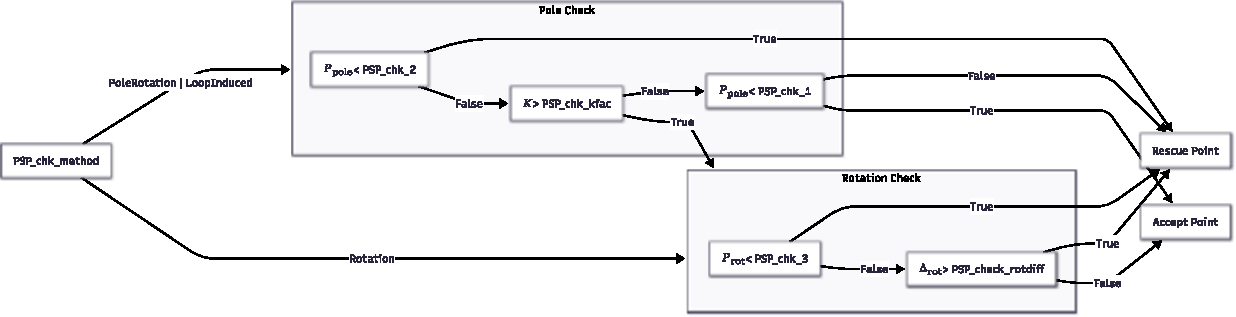
\includegraphics[scale=1.1]{figures/PSP_Check.pdf}
    \caption{Flowchart of the precision check system described in the text. The variables \texttt{PSP\_chk\_<index>} stand for \texttt{PSP\_chk\_th<index>} or \texttt{PSP\_chk\_li<index>} depending on the amplitude type.}
    \label{fig:rescue-check}
\end{figure}
\end{landscape}

\begin{landscape}
\begin{figure}
    \centering
    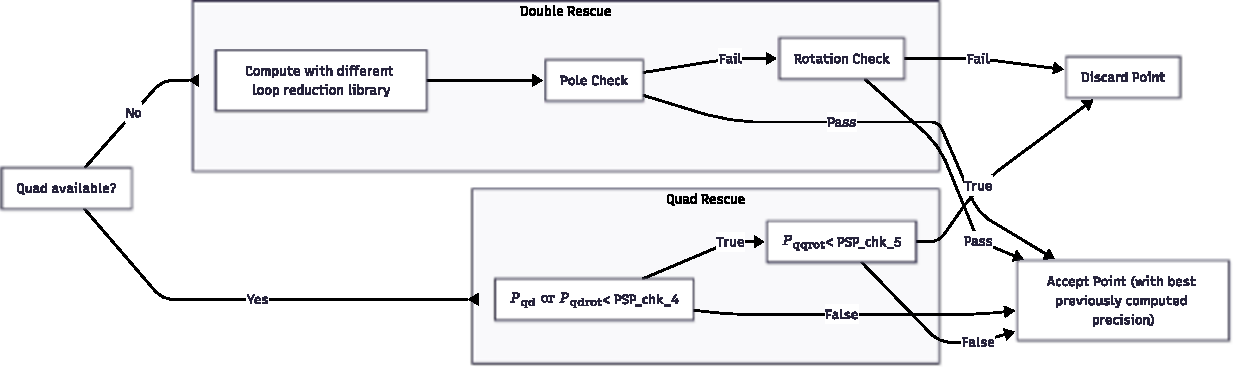
\includegraphics[scale=1]{figures/PSP_Rescue.pdf}
    \caption{Flowchart of the point rescue system described in the text. The variables \texttt{PSP\_chk\_<index>} stand for \texttt{PSP\_chk\_th<index>} or \texttt{PSP\_chk\_li<index>} depending on the amplitude type. The pole and rotation check are the ones described in Figure \ref{fig:rescue-check}.}
    \label{fig:rescue-rescue}
\end{figure}
\end{landscape}
